\documentclass{beamer}
\usepackage{xgreek}
\usepackage{xltxtra}
\usepackage{graphicx}
\useoutertheme{shadow}
\usetheme{Singapore}
\setsansfont[Mapping=tex-text]{GFS Didot}
\setmonofont[Mapping=tex-text]{DejaVu Sans Mono}
%Remove navigation symbols
\setbeamertemplate{navigation symbols}{}
%effect so overlays not yet revealed will faintly appear
\setbeamercovered{dynamic}

\title[ScorpioFS]{ScorpioFS\\Κατανεμημένο ομότιμο σύστημα αρχείων}
\author{Αντώνης Κουζούπης}
\institute{Πανεπιστήμιο Πειραιώς\\Τμήμα Πληροφορικής}
\date{\today}
\logo{
\includegraphics[scale=0.5]{images/unipi_logo.jpg}}

\begin{document}
\frame{
    \titlepage
}
\section{Εισαγωγή}
\subsection{}
\frame{
\frametitle{Τι είναι το ScorpioFS}
\begin{itemize}
\item Σύστημα αποθήκευσης αντιγράφων ασφαλείας \\ \footnotesize 
Παρέχει στο χρήστη ένα τοπικά προσαρτημένο σύστημα αρχείων το οποίο αποθηκεύει
τα περιεχόμενά του στο δίκτυο.\normalsize
\pause
\item Δίκτυο ομότιμων κόμβων \\
\footnotesize Αποτελεί ένα δίκτυο υπολογιστών που παρέχουν
στην υπηρεσία μία τοπική αποθήκη καθώς και μία λειτουργία αντιγραφής των αρχείων
μεταξύ των κόμβων για την εξασφάλιση της διαθεσιμότητας των δεδομένων.\normalsize
\pause
\item Κατανεμημένο σύστημα \\
\footnotesize Το σύστημα αποθήκευσης αρχείων είναι πλήρως αποκεντρωμένο. Όλοι οι
κόμβοι στο δίκτυο έχουν ισότιμα δικαιώματα. Κληρονομεί τα πλεονεκτήματα και τα
μειονεκτήματα των κατανεμημένων συστημάτων.\normalsize
\end{itemize}
}
\subsection{}
\frame{
\frametitle{Τα μέρη του ScorpioFS \\ (Chord)(Σκατά Τίτλος!!!)}
Το μέρος του \emph{ScorpioFS} που υλοποιεί το
Chord πρωτόκολλο. Είναι υπεύθυνο για την εύρεση των κόμβων που είναι
αποθηκευμένα τα δεδομένα, την εισαγωγή και τη διαγραφή ενός κόμβου από το
δίκτυο και τη δρομολόγηση των ερωτημάτων..
}

\frame{
\frametitle{Τα μέρη του ScorpioFS \\ (Fuse)(Σκατά Τίτλος!!!)}
Υλοποιεί το τοπικό σύστημα αρχείων που αντιλαμβάνεται ο
χρήστης. Υλοποιεί τις περισσότερες λειτουργίες ενός συστήματος αρχείων όπως
δημιουργία, διαγραφή, επεξεργασία, αντιγραφή κτλ. Χωρίζει μεγάλα αρχεία σε
μικρότερα του 1MB και επικοινωνεί με το \textbf{Chord} κομμάτι για την αποστολή
και αποδοχή δεδομένων.
}

\frame{
\frametitle{Τα μέρη του ScorpioFS \\ (Console)(Σκατά Τίτλος!!!)}
Κονσόλα διαχείρισης των κόμβων του δικτύου. Εκτελεί διάφορες λειτουργίες μαζικά
στους κόμβους όπως δημιουργία ή καταστροφή, περισυλλογή των στατιστικών.
Λειτουργεί ανεξάρτητα από το \textbf{Chord} και \textbf{Fuse} κομμάτι και
επιτελεί επικουρικό ρόλο στο σύστημα.
}

\subsection{}
\frame{
\frametitle{Σχεδιάγραμμα Δικτύου}
\begin{figure}
    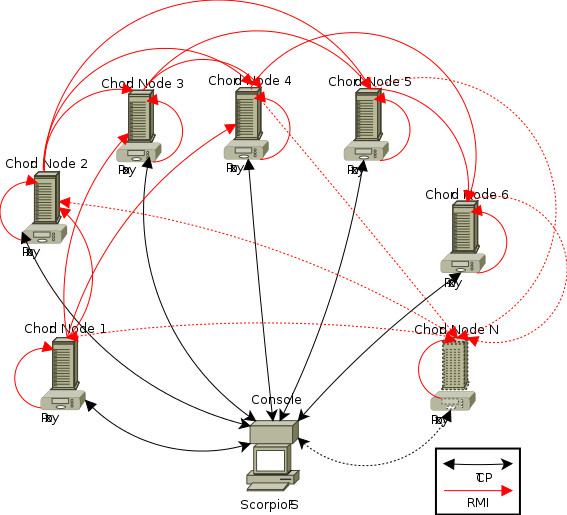
\includegraphics[scale=0.4]{images/scorpio_console.png}
\end{figure}
}

\section{Chord}

\subsection{}
\frame{
\transboxin
\frametitle{Το πρωτόκολλο Chord}
\begin{itemize}
    \item University of California, Berkeley \& MIT Laboratory for Computer
Science -- SIGCOMM'01
    \item Επεκτάσιμο πρωτόκολλο για αναζήτηση σε ένα δυναμικό peer--to--peer
σύστημα με συχνές αφίξεις και αναχωρήσεις κόμβων.
    \item Δοθέντος ενός κλειδιού το αντιστοιχίζει σε ένα κόμβο.
    \item \emph{Consistent hashing} για εξισορρόπηση του φόρτου εργασίας, κάθε κόμβος
είναι υπεύθυνος για περίπου τον ίδιο αριθμό κλειδιών, ελάχιστες μετακινήσεις
κλειδιών όταν ένας κόμβος μπαίνει ή βγαίνει από το σύστημα.
\end{itemize}
}

\frame{
\frametitle{Το πρωτόκολλο Chord}
\begin{itemize}
    \item Σε ένα σύστημα με N κόμβους, κάθε κόμβος κρατάει πληροφορία για μόνο
$\bigcirc{(\log{N})}$ άλλους κόμβους.
    \item Επιλύει όλες τις αναζητήσεις μέσω $\bigcirc{(\log{N})}$ μηνυμάτων προς
άλλους κόμβους.
    \item Το πρωτόκολλο παρέχει μία $lookup(key)$ λειτουργία που βρίσκει την IP
διεύθυνση του κόμβου που είναι υπεύθυνος για το κλειδί.
    \item Το Chord ενημερώνει τους κόμβους για τις αλλαγές των κλειδιών που
είναι υπεύθυνοι.
    \item Όταν ο N-οστός κόμβος έρθει ή φύγει από το σύστημα μόνο
$\bigcirc{(\frac{1}{N})}$ κλειδιά μετακινούνται.
\end{itemize}
}

\subsection{}
\frame{
\frametitle{Χαρακτηριστικά του Chord}
\begin{itemize}
    \item \textbf{Load balance} -- Το Chord λειτουργεί σαν κατανεμημένη
συνάρτηση κατακερματισμού διαμοιράζοντας τα κλειδιά σε όλους τους κόμβους.
    \item \textbf{Decentralization} -- Κανένας κόμβος δεν είναι πιο σημαντικός
από τους άλλους. Κατάλληλο για χαλαρά συνδεδεμένες peer--to--peer εφαρμογές.
    \item \textbf{Scalability} -- Το κόστος μιας αναζήτησης αυξάνεται
λογαριθμικά σε σχέση με το πλήθος των κόμβων.
    \item \textbf{Availability} -- Ρυθμίζει αυτόματα το δίκτυο ώστε να
``κρύψει'' από την εφαρμογή τις αποχωρήσεις και τις αφίξεις νέων κόμβων.
    \item \textbf{Flexible naming} -- Δεν θέτει κάποιο περιορισμό στη μορφή των
κλειδιών.
\end{itemize}
}

\frame{
\frametitle{Consistent Hashing}
Ένα κλειδί $\kappa$ ανατίθεται στο πρώτο κόμβο που το αναγνωριστικό του ισούται
ή ακολουθεί το $\kappa$. Ο κόμβος αυτός ονομάζεται $successor$ κόμβος του
κλειδιού $\kappa$.

\begin{figure}
    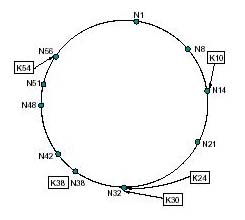
\includegraphics[scale=2]{images/chord_hashing.jpg}
\end{figure}
}

\subsection{}
\frame{
\frametitle{Finger Table}
Κάθε κόμβος $n$ κρατάει ένα πίνακα δρομολόγησης με $m (\bigcirc{(log{N})})$
εγγραφές που ονομάζεται \emph{finger table}. Το i-οστό στοιχείο του πίνακα
περιέχει το αναγνωριστικό του πρώτου κόμβου που απέχει από τον $n$ κατά
λιγότερο από $2^{i-1}$.

\begin{figure}
    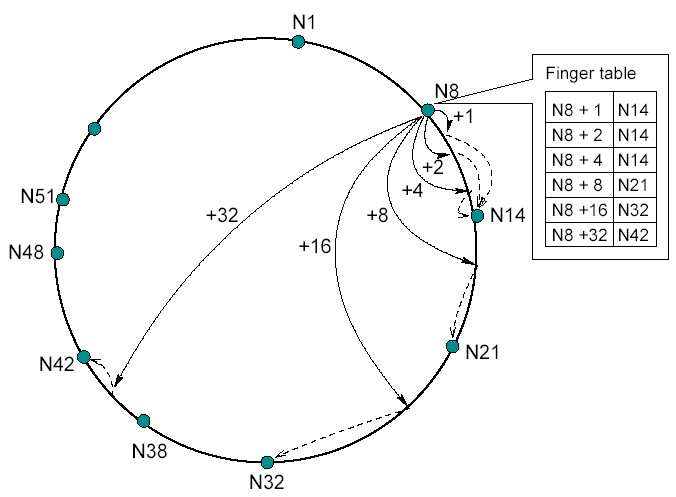
\includegraphics[scale=0.3]{images/chord_finger.png}
\end{figure}
}

\frame{
\frametitle{Finger Table}
Το πρώτο στοιχείο στον πίνακα του κόμβου $8$ είναι ο κόμβος $14$ αφού είναι ο πρώτος
κόμβος που έπεται το $(8+2^0)\mod{2^6}=9$. Αντίστοιχα, το τελευταίο στοιχείο του
πίνακα είναι ο κόμβος $42$, καθώς είναι ο πρώτος κόμβος που έπεται του
$(8+2^5)\mod{2^6}=40$.
}

\frame{
\frametitle{Finger Table}
\begin{itemize}
    \item Κάθε κόμβος κρατάει πληροφορία για ένα μικρό αριθμό κόμβων. Επίσης αυτοί
οι κόμβοι είναι οι πιο κοντινοί του.
    \item Γενικά το finger table ενός κόμβου δεν περιέχει αρκετή πληροφορία ώστε να
καθορίσει τον successor ενός τυχαίου κλειδιού $k$.
    \item Η διαδικασία για την εύρεση ενός successor μπορεί να γίνει αναδρομικά
και στους κόμβους του finger table ενός κόμβου $n$, εάν το κλειδί προς αναζήτηση
είναι πιο μακρυά από τον τελευταίο κόμβο στο finger table του κόμβου $n$.
    \item Καθώς κάθε κόμβος έχει εγγραφές σε διαστήματα της δύναμης του δύο, μπορεί
να προωθήσει μία ερώτηση τουλάχιστον στο μισό δρόμο.
\end{itemize}
}

\frame{
\frametitle{Finger Table}
Εάν υποθέσουμε ότι ο κόμβος $8$ θέλει να βρει τον successor για το κλειδί $54$.
Αφού η μεγαλύτερη εγγραφή στο finger table του κόμβου $8$ που προηγείται του $54$
είναι ο κόμβος $42$, ο κόμβος $8$ θα ρωτήσει τον κόμβο $42$ να εξυπηρετήσει την
ερώτηση.

Ο κόμβος $42$ βρίσκει ότι η μεγαλύτερη εγγραφή που προηγείται του $54$ είναι ο
κόμβος $51$. Ο κόμβος $51$ θα βρει ότι ο successor του $54$ είναι ο
κόμβος $56$. Τελικά ο κόμβος $51$ θα επιστρέψει στον κόμβο $8$ ότι ο successor
του κλειδιού $54$ είναι ο κόμβος $56$.
}

\subsection{}
\frame{
\frametitle{Εισαγωγή Κόμβου}
Ένας νέος κόμβος $n$ εισέρχεται στο σύστημα:
\begin{enumerate}
    \item Ο κόμβος $n$ καλεί όποιο κόμβο γνωρίζει και του ζητάει να του βρει τον
successor του.
    \item Ο κόμβος $n$ αντιγράφει όσα στοιχεία από το finger table του successor
του είναι μικρότερα από $n$.
    \item Ανά τακτά διαστήματα γίνεται ``stabilize'' στο δίκτυο. Ο τρέχοντας
κόμβος ρωτάει τον successor του, για τον predecessor του successor του. Με αυτό
τον τρόπο ένας νέος κόμβος γίνεται γνωστός στο δίκτυο.
    \item Κάθε κόμβος ελέγχει περιοδικά τον predecessor του για ενημερώσει τυχών
λανθασμένες εγγραφές.
\end{enumerate}
}

\frame{
\frametitle{Εισαγωγή Κόμβου}
Ο κόμβος $26$ εισέρχεται στο σύστημα μεταξύ των κόμβων $21$ και $32$. Ο κόμβος
$26$ βρίσκει τον successor του (κόμβος $32$). Ο κόμβος $26$ αντιγράφει όλα τα
κλειδιά του successor του που είναι μικρότερα από $26$. Με τη διαδικασία του
``stabilize'' ενημερώνεται ο κόμβος $21$, ότι ο successor του είναι ο κόμβος $26$

Να scan-aro και να βάλω το παράδειγμα από το paper.
}

\subsection{}
\frame{
\frametitle{Αποχώρηση Κόμβου}
Για να αυξηθεί η διαθεσιμότητα του συστήματος, κάθε κόμβος κρατάει μία λίστα από
successors ($\Omega(\log{N})$) και όχι μόνο έναν. Εάν μία κλήση προς ένα successor αποτύχει, τότε
γίνεται κλήση στον αμέσως επόμενο. Θα πρέπει να αποτύχουν όλοι οι κόμβοι για να
υπάρχει δυσλειτουργία.\\[1em]

Ένας κακόβουλος χρήστης θα μπορούσε κάνει ορισμένους κόμβους να αποτύχουν αλλά
όχι συγκεκριμένους κατ' επιλογή κόμβους.
}

\frame{
\frametitle{Αποχώρηση Κόμβου}
Η εφαρμογή που χρησιμοποιεί το Chord πρωτόκολλο, ScorpioFS, αντιγράφει τα
δεδομένα και σε άλλους κόμβους. Έτσι για τα ίδια δεδομένα είναι υπεύθυνοι
παραπάνω από ένας κόμβοι αλλά με άλλο κλειδί.\\[1em]

Μία οικειοθελής αποχώρηση μπορεί να θεωρηθεί σαν μία αποτυχία του κόμβου.
}

\section{FUSE}
\subsection{}
\frame{
\transboxin
\frametitle{Virtual File System}
\begin{itemize}
    \item Αφαιρετικό επίπεδο πάνω από ένα πιο συμπαγές σύστημα αρχείων.
    \item Επιτρέπει σε εφαρμογές χρήστη (user space) να έχουν πρόσβαση σε ένα
συμπαγές σύστημα αρχείων.
    \item Διαφανής χρήση αποθηκευτικών μέσων χωρίς ο χρήστης να καταλαβαίνει τη
διαφορά.
    \item Το VFS προσθέτει μία διεπαφή μεταξύ του πυρήνα και του συμπαγούς
συστήματος αρχείων. Συνεπώς είναι εύκολη η δημιουργία νέων συστημάτων αρχείων.
\end{itemize}
}

\subsection{}
\frame{
\frametitle{Filesystem in USErspace}
\begin{itemize}
    \item Μέρος του προγράμματος A Virtual Filesystem (AVFS), αλλά τώρα είναι
ανεξάρτητο.
    \item Ανοιχτό λογισμικό με άδεια χρήσης GNU GPL και GNU Library GPL.
    \item Διαθέσιμο για Unix-like λειτουργικά συστήματα, Linux, FreeBSD, NetBSD,
Mac OS X, OpenSolaris, GNU/Hurd.
    \item Επίσημα στον πυρήνα του Linux από την έκδοση 2.6.14
\end{itemize}
}

\frame{
\frametitle{Filesystem in USErspace}
\begin{itemize}
    \item Unix kernel module που επιτρέπει σε μη εξουσιοδοτημένους χρήστες να
δημιουργήσουν το δικό τους σύστημα αρχείων.
    \item Είναι μία ``γέφυρα'' μεταξύ του πυρήνα και της εφαρμογής του χρήστη.
    \item Χρησιμοποιεί inode cache και data buffers για βελτίωση στην ταχύτητα.
    \item Απλό API με bindings σε πολλές γλώσσες προγραμματισμού.
    \item Απλή εγκατάσταση χωρίς την μεταγλώττιση του πυρήνα.
    \item Ανάπτυξη με γνώμονα την ασφάλεια.
    \item Σταθερό!
\end{itemize}
}

\frame{
\frametitle{Filesystem in USErspace}
Εφαρμογές που χρησιμοποιούν το FUSE:
\begin{itemize}
    \item Wuala
    \item SSHFS
    \item NTFS-3G
    \item TrueCrypt
    \item vmware-mount
    \item ...
\end{itemize}
}

\subsection{}
\frame{
\frametitle{Filesystem in USErspace}
Η δομή του FUSE:
\begin{figure}
    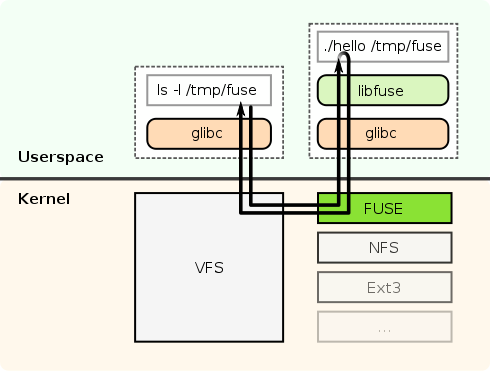
\includegraphics[scale=0.5]{images/FUSE_struct.svg.png}
\end{figure}
}

\frame{
\frametitle{FUSE-J}
\begin{itemize}
    \item Java API που παρέχει στο χρήστη bindings για το FUSE.
    \item Χρησιμοποιεί το framework Java Native Interface (JNI), που επιτρέπει
σε κλάσεις Java να καλέσουν ή να καλεστούν (από) native προγράμματα γραμμένα σε
γλώσσες όπως C, C++, assembly.
    \item Ανοιχτό λογισμικό με άδεια GNU Library GPL.
\end{itemize}
}

\section{ScorpioFS}
\subsection{}
\frame{
\transboxin
\frametitle{Αναπαράσταση Αρχείων}
\begin{itemize}
    \item Τα αρχεία χωρίζονται σε chunks μεγέθους 1MB.
    \item Τα δεδομένα είναι σε μορφή πίνακα από bytes.
    \item Κάθε chunk υλοποιείται από ένα instance της κλάσης \emph{DataObject}.
    \item Όλα τα chunks -- DataObject που αποτελούν ένα αρχείο κρατούνται στην
κλάση \emph{DataList}. Κάθε αρχείο έχει ένα instance αυτής της κλάσης.
\end{itemize}
}

\frame{
\frametitle{Αναπαράσταση Αρχείων}
\begin{itemize}
    \item Κάθε ``κόμβος'' στο ScorpioFS αποτελεί ένα instance της κλάσης
\emph{FsNode}.
    \item Κρατάει διάφορες πληροφορίες για έναν ``κόμβο'' όπως όνομα, μέγεθος,
τον πατέρα του κόμβου, \emph{DataList}, κτλ
    \item Όλοι οι κόμβοι -- \emph{FsNode} s κρατούνται στην κλάση \emph{FsTree}.
    \item Το \emph{FsTree} είναι μία συλλογή από \emph{FsNode} s. Επομένως η
κλάση \emph{FsTree} υλοποιεί το σύστημα αρχείων.
    \item Η κλάση \emph{FsTree} είναι serializable, αποθηκεύεται και στέλνεται
στο δίκτυο σαν ένα κανονικό αρχείο.
\end{itemize}
}

\frame{
\frametitle{Αναπαράσταση Αρχείων}
\begin{figure}
    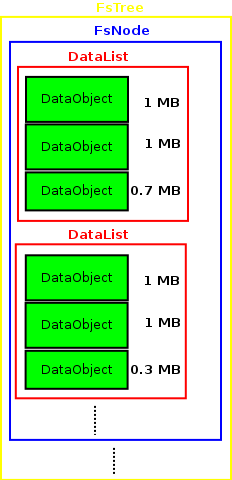
\includegraphics[scale=0.4]{images/file_system.png}
\end{figure}
}

\subsection{}
\frame{
\frametitle{Έναρξη ScorpioFS}
\begin{itemize}
    \item Υπάρχει τοπικά ένα αρχείο το οποίο περιέχει τα keys από τα chunks από
τα οποία αποτελείται το \emph{FsTree}.
    \item Το αρχείο αυτό είναι κρυπτογραφημένο με AES-128 αλγόριθμο
κρυπτογράφησης και PBKDF2 (Password-Based Key Derivation Function 2) συνάρτηση
παραγωγής κλειδιού.
    \item Αρχικά η εφαρμογή αποκρυπτογραφεί το αρχείο και ανακτά από το δίκτυο
τα chunks του \emph{FsTree}.
    \item Κάνει deserialize το αρχείο, προσαρτάται ένας κατάλογος και ``χτίζει''
εκεί το σύστημα αρχείων.
\end{itemize}
}

\frame{
\frametitle{Λήξη ScorpioFS}
\begin{itemize}
    \item Γίνεται serialize το \emph{FsTree}.
    \item Εάν είναι μεγαλύτερο από 1 ΜΒ, σπάει σε μικρότερα chunks και
στέλνονται στο δίκτυο όπως τα κανονικά αρχεία.
    \item Αποθηκεύονται τα keys των παραπάνω chunks σε ένα αρχείο.
    \item Κρυπτογραφείται το αρχείο και αποθηκεύεται τοπικά.
    \item Αποπροσαρτάται ο τοπικός κατάλογος και σταματάει το πρόγραμμα.
\end{itemize}
}
\subsection{}
\frame{
\frametitle{Εγγραφή ενός αρχείου}
\begin{itemize}
    \item Κλήση της κατάλληλης μεθόδου που επικοινωνεί με το FUSE για την
εγγραφή του αρχείου στο σύστημα αρχείων.
    \item Δημιουργία ενός νέου \emph{FsNode} και αρχικοποίησή του.
    \item Δημιουργία \emph{DataObject} s με μέγεθος 1 MB.
    \item Δημιουργία \emph{DataList} με τα παραπάνω \emph{DataObject} s.
    \item Προσάρτηση του τρέχοντα κόμβου -- \emph{FsNode} στο κατάλληλο σημείο
του \emph{FsTree}.
    \item Αφού κλείσει ο file descriptor για το συγκεκριμένο αρχείο, τότε
ξεκινάει η διαδικασία για την αποστολή του στο δίκτυο.
\end{itemize}
}

\frame{
\frametitle{Εγγραφή ενός αρχείου}
\begin{itemize}
    \item Δημιουργείται το SHA-1 hash του \emph{DataObject}.
    \item Ο κόμβος συμβουλεύεται το Finger Table του και σύμφωνα με το παραπάνω
hash αποφασίζει ποιος κόμβος είναι υπεύθυνος για αυτό.
    \item Επικοινωνεί με τον κόμβο αυτό με RMI κλήση και του στέλνει το chunk.
\end{itemize}
}

\frame{
\frametitle{Ανάγνωση ενός αρχείου}
\begin{itemize}
    \item Καλείται η $read$ μέθοδος από το FUSE.
    \item Αν το συγκεκριμένο \emph{DataObject} υπάρχει στην τοπική αποθήκη του
κόμβου τότε διαβάζεται από εκεί.
    \item Διαφορετικά μέσω της λειτουργίας που ορίζει το Chord πρωτόκολλο,
ο κόμβος βρίσκει ποιος κόμβος είναι υπεύθυνος για το chunk αυτό.
    \item Μέσω RMI κλήσης φέρνει το chunk και το ανοίγει.
    \item Υπάρχει η δυνατότητα για την ανάκτηση συγκεκριμένων chunks και όχι
όλου του αρχείου.
\end{itemize}
}

\subsection{}
\frame{
\frametitle{Αντιγραφή Αρχείων}
\begin{itemize}
    \item Ανά τακτά χρονικά διαστήματα -- 5 δευτερόλεπτα -- ξεκινάει η
διαδικασία αντιγραφής αρχείων μεταξύ των κόμβων στο δίκτυο.
    \item Για κάθε ένα αρχείο που έχει στην αποθήκη του ο κόμβος, υπολογίζεται
πάλι το SHA-1 hash του.
    \item Αναζητάται ο υπεύθυνος κόμβος για το νέο πλέον key και μέσω RMI κλήσης
αντιγράφεται σε αυτόν.
    \item Αν ο νέος υπεύθυνος κόμβος δεν είναι γνωστός για τον τρέχοντα τότε
ψάχνει αναδρομικά.
    \item Η παραπάνω διαδικασία περιορίζεται από ένα Replication Factor.
\end{itemize}
}

\frame{
\frametitle{Κονσόλα Διαχείρισης}
\begin{itemize}
    \item Έχει επικουρικό ρόλο στο σύστημα. Βοηθάει για τη μαζική εκτέλεση ενεργειών
στους κόμβους.
    \item Αρχιτεκτονική πελάτη--εξυπηρετητή χρησιμοποιώντας το TCP πρωτόκολλο
επικοινωνίας.
    \item Η κονσόλα διαχείρισης στέλνει μηνύματα στους κόμβους.
    \item Σε κάθε Chord κόμβο υπάρχει ένας proxy εξυπηρετητής που λαμβάνει τα
μηνύματα και τα προωθεί.
    \item Στην κονσόλα διαχείρισης υπάρχει ένας πολυνηματικός εξυπηρετητής που
λαμβάνει τα μηνύματα των κόμβων.
\end{itemize}
}

\frame{
\frametitle{Κονσόλα Διαχείρισης}
Οι λειτουργίες που προσφέρει η κονσόλα διαχείρισης είναι:
\begin{itemize}
    \item Δημιουργία κόμβων μεμονωμένα ή μαζικά.
    \item Σταμάτημα κόμβων μεμονωμένα ή μαζικά.
    \item Απαρίθμηση των ενεργών κόμβων στο δίκτυο.
    \item Συγκέντρωση και εξαγωγή σε αρχεία διάφορων στατιστικών από τους κόμβους.
\end{itemize}
}
\section{Πειράματα}
\subsection{}
\frame{
\frametitle{Αντιγραφή Αρχείων}
\begin{figure}
    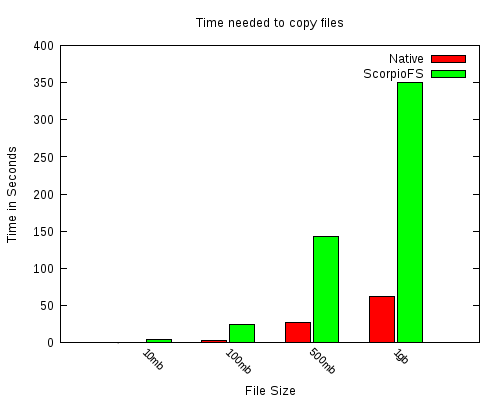
\includegraphics[scale=0.5]{../statistics/copy_files.png}
\end{figure}
}

\frame{
\frametitle{Διαγραφή Αρχείων}
\begin{figure}
    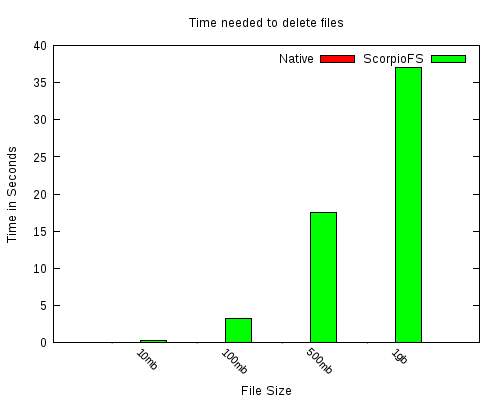
\includegraphics[scale=0.5]{../statistics/delete_files.png}
\end{figure}
}
\section{Εκτέλεση}
\section{Επίδειξη}
\section{Μελλοντική Εργασία}
\end{document}
